\section{Propagation of the Particles and Light}
After generation, IceCube simulated events require two types of \emph{propagation}.
The first, the propagation of charged leptons, produces the energy losses in the detector due to continuous and stochastic emissions.
These energy losses are then used to produce photons that may be propagated through the detector using models of the Antarctic glacier.

\label{sec:propagation}

\subsection{Lepton Propagation with PROPOSAL}
\label{subsec:proposal}

\begin{figure}
\centering
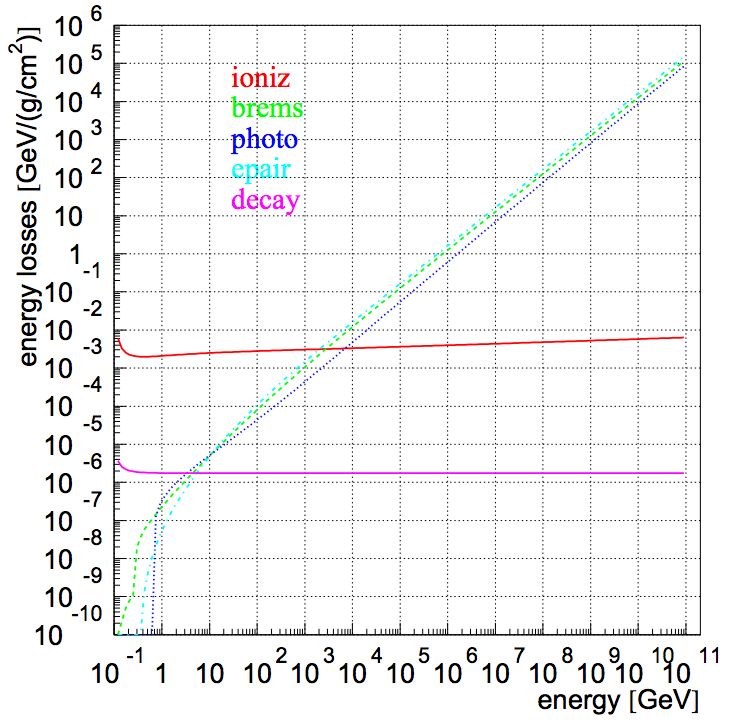
\includegraphics[width=0.6\linewidth]{discrete_emissions_MMC.png}
\caption{Average energy losses ($\mathtt{\frac{-dE}{dX}}$) for a muon in ice. At very low energies, ionization losses dominate. Above approximately 1 TeV, pair production and photonuclear effects become more important. Image taken from \cite{Dima-MMC}}
\label{fig:discrete_emissions}
\end{figure}

The propagation of leptons in IceCube is performed using \emph{PROPOSAL}, a software module which contains tools to simulate the propagation of leptons and hadrons with ionization, electron pair-production, bremsstrahlung, photonuclear interactions, and decay processes \cite{PROPOSAL}.
The Cherenkov light output from daughter particles in each case is handled by a parametrization of the associated energy deposition for a given true particle energy as shown in Figure~\ref{fig:discrete_emissions}.

PROPOSAL propagates the charged particles through the detector, producing a series of energy emissions associated with each propagated particle.
The omdule takes into account the position of the particle and uses separate cross sections for glacial ice and the underlying bedrock 300 m below IceCube.

\subsection{CLSim for Photon Propagation}
\label{subsec:clsim}
Once the energy deposition at each position is calculated, the resulting photons must be produced and propagated. 
There exist two modules which can handle this: Photon Propagation Code \emph{PPC} and OpenCL Simulation Code \emph{CLSim}. 
The differences are largely of implementation details and both have been verified to give identical results.
Only the latter, CLSim, will be discussed here.

CLSim is a code designed to propagate emitted photons using ray tracing algorithms \cite{PPC}.
The independence of the individual photons is leveraged to perform the propagation of all photons in parallelized calculations using the OpenCL programming language \cite{OpenCL}.
Photons are then propagated through the ice with the current best-fit knowledge about the scattering and absorption properties, continuing until either absorbed or until they reach a DOM.
Photons which reach DOMs are stored.

The propagation of individual photons is efficient at low energies, where the scattering of individual photons is important.
At energies above a few hundred GeV, the light yield is large enough that the propagation of individual photons is both excessively costly as well as unnecessary.
In those cases, a feature known as \emph{oversizing} is used by setting a \emph{oversize factor}, $N_{OS}$.
The oversize factor, often set to 5 for IceCube simulations above 1 TeV, allows for the production of "weighted photons" representing photon bundles with size proportional to $N^2_{OS}$, significantly reducing the computational power necessary for large numbers of photons.
In order to compensate for the bundling of photons, the effective radius of the DOM is also increased by $N_{OS}$.

Oversizing is efficient for the simulation of high energy events with large numbers of photon.
This breaks down at GeV energies, where the photon flux from an event is low and scattering or absorption of individual photons matters.
Because of the complications associated with oversizing at low energies, most simulations of DeepCore events are done with the oversizing features disabled.

\subsection{Angular Acceptance and Hole Ice}
\label{subsec:holeice_sim}

\begin{figure}
\centering
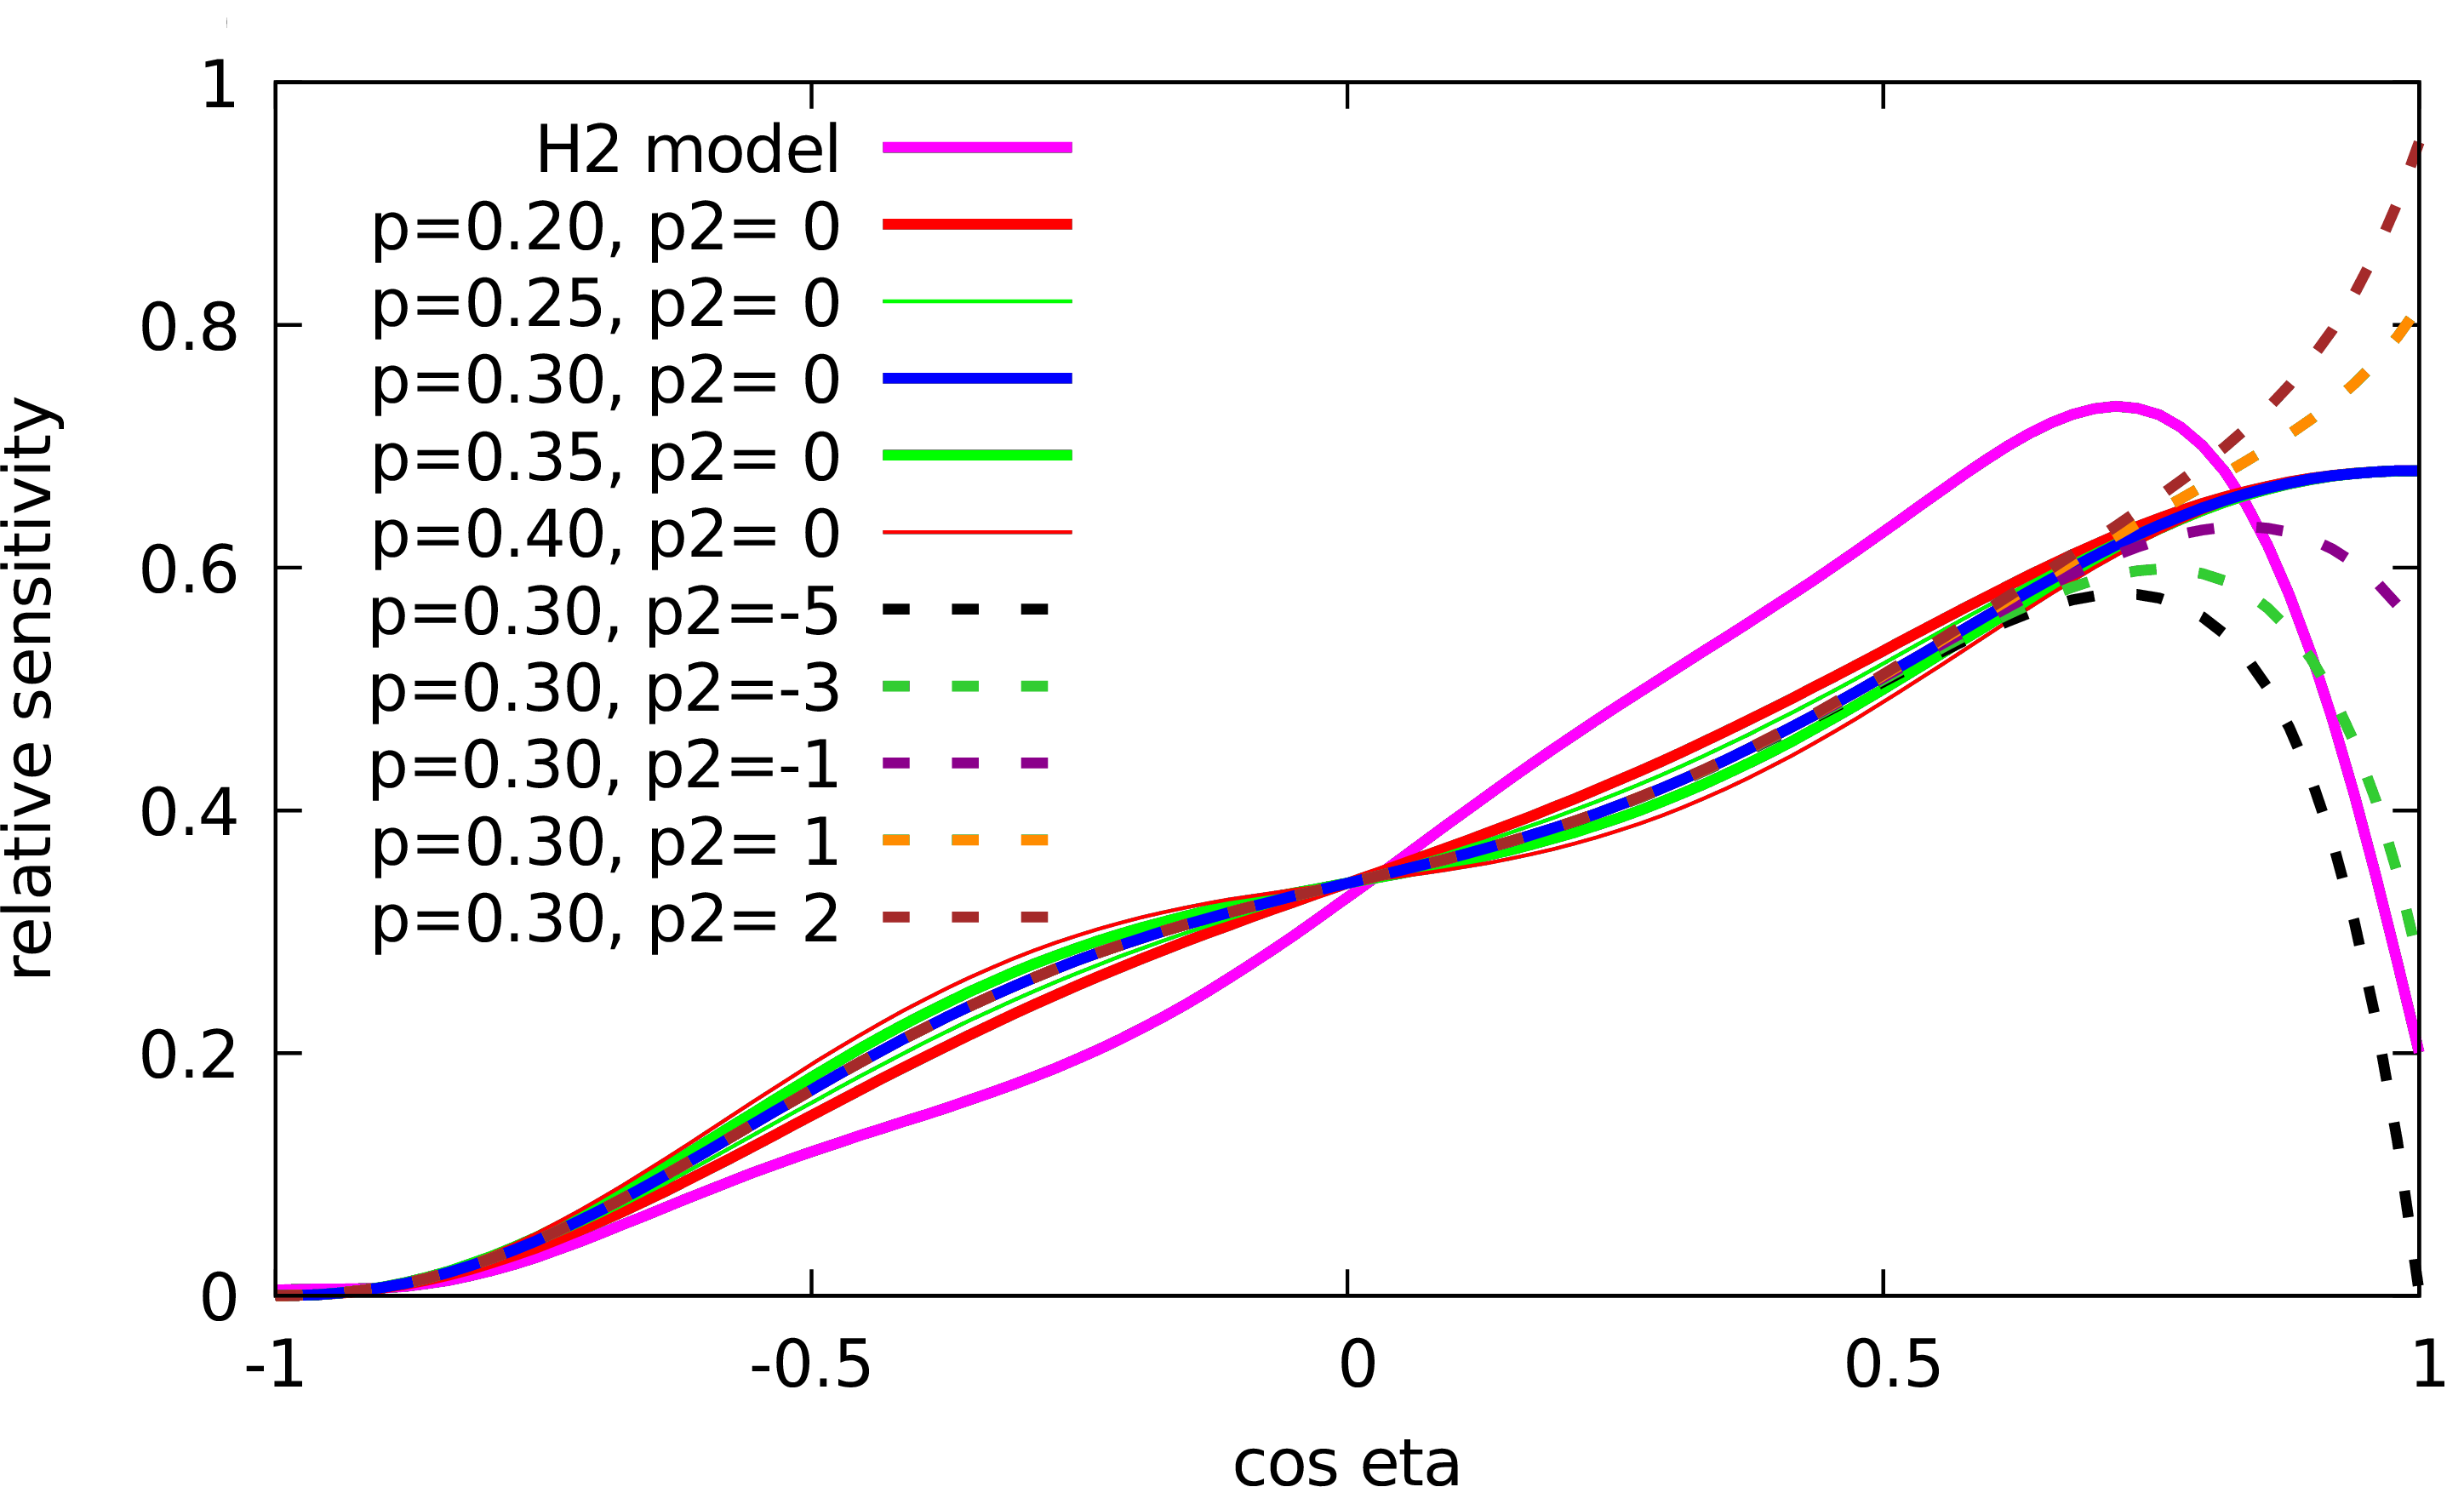
\includegraphics[width=0.7\textwidth]{angular_acceptance.png} 
\caption{Examples of the angular acceptance models used by IceCube. The relative sensitivity as a function of arrival direction is shown with cos(eta)=-1 indicating the back of the PMT and cos(eta)=1 the face. The variation of the acceptance model used for this search is shown using by varying two parameters in the model. The 'p' parameter primarily controls the acceptance at the side of the DOM while the 'p2' parameter controls the acceptance from the forward region. A second model, H2, is also shown.}
\label{fig:angular_acceptance}
\end{figure}

When photons reach the surface of a DOM, the \emph{angular acceptance} is applied in order to model the hole ice.
This acceptance, calculated from a combination of lab and in-situ measurements, represents the PMT efficiency as a function of the photon arrival direction.
The acceptance has a negligible efficiency for photons arriving from the back of the PMT and high efficiency for photons reaching the face of the PMT as shown in Figure~\ref{fig:angular_acceptance}.
All other directions follow a curve between these two points.
The angular acceptance model used in this thesis uses an empirical form fit to flasher data with two free parameters, as shown in Figure~\ref{fig:angular_acceptance}.
The most forward direction in the PMT, shown with $cos(\eta)$ = 1, is most affected by the bubble column (see Section~\ref{sec:hole_ice}). 

